\documentclass[12pt,a4paper,oneside]{report}

% ================= PACKAGES =================
\usepackage[a4paper,margin=1in]{geometry}
\usepackage[utf8]{inputenc}
\usepackage[T1]{fontenc}
\usepackage{graphicx}
\usepackage{booktabs}
\usepackage{array}
\usepackage{longtable}
\usepackage{amsmath,amssymb}
\usepackage{caption}
\usepackage{subcaption}
\usepackage{float}
\usepackage{enumitem}
\usepackage{xcolor}
\usepackage{fancyhdr}
\usepackage{titlesec}
\usepackage{setspace}
\usepackage{listings}
\usepackage{tikz}
\usetikzlibrary{shapes.geometric,arrows.meta,positioning,fit,backgrounds}
\usepackage[hidelinks,colorlinks=true,linkcolor=black,citecolor=black,urlcolor=blue]{hyperref}
\usepackage[nottoc]{tocbibind}
\usepackage{multirow}

% ================= PAGE STYLE =================
\onehalfspacing
\setlength{\headheight}{14.5pt}
\pagestyle{fancy}
\fancyhf{}
\fancyhead[L]{\small\leftmark}
\fancyfoot[C]{\thepage}
\renewcommand{\headrulewidth}{0.4pt}

\titleformat{\chapter}[display]
  {\normalfont\bfseries\Large}{\chaptertitlename\ \thechapter}{10pt}{\Huge}
\titlespacing*{\chapter}{0pt}{-20pt}{20pt}

% ================= LISTINGS STYLE =================
\definecolor{codebg}{RGB}{245,245,245}
\definecolor{codekeyword}{RGB}{0,0,180}
\definecolor{codecomment}{RGB}{95,130,95}
\definecolor{codestring}{RGB}{160,30,30}

\lstdefinestyle{pythonstyle}{
    backgroundcolor=\color{codebg},
    basicstyle=\ttfamily\footnotesize,
    keywordstyle=\color{codekeyword}\bfseries,
    commentstyle=\color{codecomment}\itshape,
    stringstyle=\color{codestring},
    numbers=left,
    numberstyle=\tiny\color{gray},
    numbersep=6pt,
    breaklines=true,
    breakatwhitespace=false,
    frame=single,
    rulecolor=\color{gray!40},
    tabsize=4,
    showstringspaces=false,
    language=Python
}
\lstset{style=pythonstyle}

% ================= TITLE PAGE INFO =================
\newcommand{\thesistitle}{Explainable Crop Disease Diagnosis Using Xception with LLM-Based Natural Language Decision Support for Bangladeshi Crops}
\newcommand{\authorname}{[Author Name]}
\newcommand{\studentid}{[Student ID]}
\newcommand{\supervisorname}{[Supervisor Name, Designation]}
\newcommand{\departmentname}{Department of Computer Science and Engineering}
\newcommand{\universityname}{[University Name]}
\newcommand{\submissiondate}{[Month, Year]}

\begin{document}

% ============================================================
% TITLE PAGE
% ============================================================
\begin{titlepage}
\centering
\vspace*{0.5cm}
{\LARGE \bfseries \thesistitle \par}
\vspace{1.2cm}
{\large A thesis submitted in partial fulfillment of the requirements\\ for the degree of\par}
\vspace{0.3cm}
{\large \bfseries Master of Science in Computer Science and Engineering \par}
\vspace{1.5cm}

{\large By \par}
\vspace{0.2cm}
{\large \bfseries \authorname \par}
{\large \studentid \par}

\vspace{1.8cm}
{\large Supervised by \par}
\vspace{0.2cm}
{\large \bfseries \supervisorname \par}

\vfill

\begin{figure}[H]
\centering

\begin{tikzpicture}
\node[draw, align=center, minimum width=3.2cm, minimum height=3.2cm, rounded corners, thick] (logo) {\Large\textbf{Univ.}\\\textbf{Logo}};
\end{tikzpicture}
\end{figure}

\vfill
{\large \departmentname \par}
{\large \universityname \par}
{\large \submissiondate \par}

\end{titlepage}

% ============================================================
% DECLARATION
% ============================================================
\chapter*{Declaration}
\addcontentsline{toc}{chapter}{Declaration}
I hereby declare that this thesis titled \textit{``\thesistitle''} is my own original work, carried out under the
supervision of \supervisorname{}, and has been submitted in partial fulfillment of the requirements for the degree
of Master of Science in Computer Science and Engineering at \universityname{}. All sources of information used in
this thesis have been duly acknowledged. This work has not been submitted, in whole or in part, for any other
degree or professional qualification.

\vspace{2cm}
\noindent\textbf{\authorname{}}\\
\studentid{}\\
\departmentname{}\\
\submissiondate{}

% ============================================================
% CERTIFICATE
% ============================================================
\chapter*{Certificate}
\addcontentsline{toc}{chapter}{Certificate}
This is to certify that the thesis titled \textit{``\thesistitle''}, submitted by \authorname{}
(\studentid{}), has been carried out under my supervision. This work, to the best of my knowledge, is an
original piece of research and is recommended for submission in partial fulfillment of the requirements for the
degree of Master of Science in Computer Science and Engineering.

\vspace{2cm}
\noindent\textbf{\supervisorname{}}\\
Supervisor\\
\departmentname{}\\
\universityname{}

% ============================================================
% ACKNOWLEDGEMENT
% ============================================================
\chapter*{Acknowledgement}
\addcontentsline{toc}{chapter}{Acknowledgement}
I would like to express my sincere gratitude to my supervisor, \supervisorname{}, for the continuous guidance,
patience, and valuable feedback throughout this research. I am also thankful to the faculty members and staff of
the \departmentname{} at \universityname{} for providing the resources and environment necessary to complete this
work. I extend my appreciation to my peers for their insightful discussions, and finally to my family for their
unwavering support and encouragement throughout this journey.

% ============================================================
% ABSTRACT
% ============================================================
\chapter*{Abstract}
\addcontentsline{toc}{chapter}{Abstract}
Crop diseases pose a persistent threat to food security in Bangladesh, where a substantial share of the workforce
depends directly on agriculture. Deep learning has shown strong promise for automated, image-based crop disease
diagnosis, but the black-box nature of convolutional neural networks (CNNs) limits farmer and agronomist trust in
their predictions. This thesis presents an \textbf{explainable and intelligent crop disease diagnosis framework}
that integrates a fine-tuned \textbf{Xception} convolutional neural network with two complementary
\textbf{Explainable Artificial Intelligence (XAI)} techniques -- \textbf{Gradient-weighted Class Activation
Mapping (Grad-CAM)} and \textbf{SHapley Additive exPlanations (SHAP)} -- and a \textbf{Large Language Model (LLM)}
based natural-language decision-support module.

The proposed system was trained and evaluated on the New Bangladeshi Crop Disease dataset, comprising
\textbf{13,024} leaf images across \textbf{14} disease/health classes spanning four major Bangladeshi crops: Corn,
Potato, Rice, and Wheat. Using a two-phase transfer-learning strategy (head-only training followed by fine-tuning
of the top Xception blocks), the model achieved an overall test accuracy of \textbf{92.27\%}, a macro-averaged
F1-score of \textbf{0.911}, a weighted F1-score of \textbf{0.923}, and a macro-averaged ROC-AUC of \textbf{0.997}
across all 14 classes on a held-out test set of 1,954 images. Grad-CAM and SHAP explanations were compared and
found to largely agree on the diseased leaf regions driving each prediction, supporting the reliability of the
classifier's decision process. A prompt-engineering pipeline automatically converts the model's structured
output (predicted class, confidence score, and XAI-derived visual cues) into a plain-language report covering
disease explanation, confidence interpretation, recommended treatment, and preventive measures, with support for
OpenAI GPT, local Llama-3/Gemma models, or a rule-based template fallback for fully offline operation. The
complete pipeline was deployed as an interactive Streamlit web application, allowing a user to upload a leaf
photograph and immediately receive a classification, a visual explanation, and a farmer-friendly diagnostic
report. The results demonstrate that combining a high-accuracy CNN classifier with XAI and LLM-based natural
language generation can substantially improve the transparency, interpretability, and practical usability of
AI-assisted crop disease diagnosis for Bangladeshi agriculture.

\vspace{0.5cm}
\noindent\textbf{Keywords:} Crop Disease Diagnosis, Xception, Transfer Learning, Explainable AI, Grad-CAM, SHAP,
Large Language Models, Natural Language Generation, Precision Agriculture, Bangladesh.

% ============================================================
% TOC / LOF / LOT
% ============================================================
\tableofcontents
\listoffigures
\listoftables

\chapter*{List of Abbreviations}
\addcontentsline{toc}{chapter}{List of Abbreviations}
\begin{table}[H]
\centering
\begin{tabular}{ll}
\toprule
\textbf{Abbreviation} & \textbf{Full Form} \\
\midrule
AI & Artificial Intelligence \\
AUC & Area Under the Curve \\
CNN & Convolutional Neural Network \\
DAE & Department of Agricultural Extension \\
F1 & F1-score (harmonic mean of precision and recall) \\
Grad-CAM & Gradient-weighted Class Activation Mapping \\
GPT & Generative Pre-trained Transformer \\
LLM & Large Language Model \\
ReLU & Rectified Linear Unit \\
ROC & Receiver Operating Characteristic \\
SHAP & SHapley Additive exPlanations \\
XAI & Explainable Artificial Intelligence \\
\bottomrule
\end{tabular}
\end{table}

% ============================================================
% CHAPTER 1: INTRODUCTION
% ============================================================
\chapter{Introduction}
\label{ch:introduction}

\section{Background and Motivation}
Agriculture remains a cornerstone of Bangladesh's economy and food security, employing a large fraction of the
population and contributing significantly to the national GDP. Rice, wheat, potato, and corn (maize) are among
the most widely cultivated crops in the country, and their productivity is frequently undermined by fungal,
bacterial, and viral diseases that spread rapidly under Bangladesh's humid, subtropical climate. Timely and
accurate disease identification is critical: early diagnosis allows farmers to apply targeted treatment before an
outbreak spreads across a field, reducing both crop loss and the indiscriminate use of chemical pesticides.

Traditionally, disease diagnosis has relied on manual inspection by farmers or agricultural extension officers,
a process that is time-consuming, subjective, and dependent on the availability of trained experts -- a resource
that is often scarce in rural areas. The widespread availability of smartphones and the rapid advancement of deep
learning, particularly Convolutional Neural Networks (CNNs), have opened new possibilities for automated,
image-based crop disease diagnosis that can be deployed directly in the field.

However, deep learning models are frequently criticized as ``black boxes'': while they can achieve high
classification accuracy, they provide little insight into \textit{why} a particular prediction was made. This
opacity is a significant barrier to adoption in agriculture, where farmers and agronomists need to understand and
trust a diagnosis before acting on it -- particularly when the recommended action (e.g., applying a fungicide)
has a real economic and environmental cost. Explainable Artificial Intelligence (XAI) techniques, such as
Grad-CAM and SHAP, address this gap by highlighting the image regions and features that most influenced a
model's decision. Separately, the recent emergence of capable Large Language Models (LLMs) offers a new
opportunity: translating a model's structured, technical output into natural, farmer-friendly language that
explains the diagnosis and recommends concrete next steps.

This thesis is motivated by the observation that no single component -- an accurate classifier, a visual
explanation, or a natural-language report -- is sufficient on its own to build a trustworthy, usable, decision-support
tool for Bangladeshi farmers. Instead, this work proposes an integrated framework that combines all three: an
Xception-based classifier for accurate diagnosis, Grad-CAM and SHAP for visual interpretability, and an LLM-based
module for natural-language decision support.

\section{Problem Statement}
Existing crop disease detection systems in the literature predominantly focus on maximizing classification
accuracy, with comparatively little attention paid to (i) the interpretability of the model's decisions, and
(ii) the practical usability of the output for non-expert end users such as smallholder farmers. Furthermore,
very few studies address disease classification specifically for crop varieties and disease presentations common
in Bangladesh, and fewer still combine visual explainability with natural-language decision support in a single,
deployable framework. This creates a gap between what deep learning models can technically achieve and what is
practically useful and trustworthy for the intended end users. This thesis addresses that gap by developing an
explainable, LLM-supported crop disease diagnosis framework tailored to Bangladeshi crops.

\section{Research Aim}
The aim of this research is to develop an explainable AI-powered crop disease diagnosis framework that combines
Xception, Explainable AI, and Large Language Models to improve the accuracy, interpretability, and practical
usability of disease diagnosis for Bangladeshi agriculture.

\section{Research Objectives}
The main objective of this research is:
\begin{quote}
To develop an explainable and intelligent crop disease diagnosis system for Bangladeshi crops by integrating the
Xception deep learning model with Explainable Artificial Intelligence (XAI) techniques and a Large Language Model
(LLM) to provide accurate disease classification, interpretable predictions, and natural-language decision
support for farmers and agricultural professionals.
\end{quote}

The specific objectives of this research are as follows:
\begin{enumerate}[label=\arabic*.]
    \item To develop a deep learning-based crop disease classification model using the Xception architecture.
    \item To evaluate the performance of the proposed model using standard metrics such as accuracy, precision,
          recall, F1-score, and confusion matrix.
    \item To integrate Explainable AI techniques (Grad-CAM and SHAP) to visualize and interpret the regions and
          features influencing disease predictions.
    \item To develop an LLM-based natural language explanation module that converts model predictions and XAI
          outputs into easy-to-understand diagnostic reports.
    \item To generate disease management recommendations, preventive measures, and treatment suggestions based
          on the predicted crop disease.
    \item To assess the effectiveness of the proposed explainable decision-support framework for improving
          transparency, usability, and trust in AI-assisted crop disease diagnosis.
\end{enumerate}

\section{Expected Contributions}
This thesis makes the following contributions:
\begin{itemize}
    \item An accurate Xception-based crop disease classifier, fine-tuned specifically on crops and disease
          classes relevant to Bangladeshi agriculture.
    \item Visual explanations using Grad-CAM and SHAP that reveal why the model made a given prediction, with a
          qualitative comparison of the two techniques.
    \item LLM-generated explanations that translate technical model outputs into farmer-friendly, natural
          language.
    \item Decision support in the form of automatically generated, disease-specific treatment and prevention
          recommendations.
    \item A complete, deployable framework (including an interactive web application) that enhances the trust,
          transparency, and usability of AI in agricultural disease diagnosis.
\end{itemize}

\section{Scope and Limitations}
This research focuses on image-based diagnosis of 14 disease/health classes across four crops (Corn, Potato,
Rice, and Wheat) using the New Bangladeshi Crop Disease dataset. The scope is limited to single-leaf image
classification under the lighting, background, and image-quality conditions represented in this dataset; it does
not address whole-plant, canopy-level, or multi-leaf diagnosis, nor does it cover pest infestations or nutrient
deficiencies that are not represented as classes in the dataset. The LLM-based decision-support module is
grounded in a compact, illustrative agronomic knowledge base and is intended as a decision-\emph{support} tool
rather than a replacement for professional agronomic advice; outputs should ideally be reviewed by a qualified
agronomist before field application, particularly in a production deployment.

\section{Thesis Organization}
The remainder of this thesis is organized as follows. \textbf{Chapter 2} reviews related work in deep
learning-based crop disease detection, transfer learning architectures, explainable AI, and the use of large
language models for decision support. \textbf{Chapter 3} describes the proposed methodology, including the
dataset, preprocessing pipeline, model architecture, training procedure, XAI techniques, and the LLM-based
natural language decision-support module. \textbf{Chapter 4} presents the experimental results, including
classification performance, confusion matrix and ROC-AUC analysis, and qualitative comparison of Grad-CAM and
SHAP explanations, along with sample LLM-generated reports. \textbf{Chapter 5} concludes the thesis with a
summary of findings, limitations, and directions for future work.

% ============================================================
% CHAPTER 2: LITERATURE REVIEW
% ============================================================
\chapter{Literature Review}
\label{ch:litreview}

\section{Deep Learning for Plant and Crop Disease Detection}
The application of deep learning to plant disease detection gained significant momentum following the work of
Mohanty et al.~\cite{mohanty2016}, who demonstrated that a CNN trained on the PlantVillage dataset could classify
26 diseases across 14 crop species with high accuracy directly from leaf images, establishing image-based deep
learning as a viable alternative to manual disease diagnosis. Ferentinos~\cite{ferentinos2018} extended this line
of work by systematically comparing several CNN architectures (including AlexNet, VGG, and GoogLeNet variants)
across a large dataset of plant leaf images, reporting that deeper architectures generally achieved higher
classification accuracy, but at increased computational cost. These early studies established the core paradigm
followed by most subsequent work: treat disease diagnosis as an image classification problem and apply
increasingly sophisticated CNN architectures pretrained on large natural-image datasets such as ImageNet
\cite{deng2009imagenet}.

Since then, a large body of work has applied transfer learning with architectures such as VGG-16
\cite{simonyan2014vgg}, ResNet \cite{he2016resnet}, and Xception \cite{chollet2017xception} to a wide range of
crop-specific disease datasets, generally reporting that transfer learning from ImageNet substantially improves
accuracy and reduces the amount of labeled data required, compared with training a CNN from scratch. However,
much of this literature is evaluated on curated, relatively homogeneous datasets (such as PlantVillage) that may
not reflect the diversity of leaf appearances, disease presentations, and image-capture conditions found in a
specific regional agricultural context such as Bangladesh.

\section{Transfer Learning and the Xception Architecture}
Xception, proposed by Chollet~\cite{chollet2017xception}, extends the Inception family of architectures by
replacing standard Inception modules with \textit{depthwise separable convolutions}, in which spatial and
cross-channel correlations are decoupled into separate convolution operations. This design substantially reduces
the number of parameters relative to comparably deep architectures while maintaining or improving representation
capacity, making Xception an attractive backbone for transfer learning in resource-constrained deployment
scenarios such as agricultural field applications. In transfer learning, a network pretrained on a large, generic
image dataset (typically ImageNet~\cite{deng2009imagenet}) is repurposed for a new, often smaller, target task by
replacing the final classification layer(s) and fine-tuning some or all of the network's weights on the target
data. A common strategy -- and the one adopted in this thesis -- is to first train only the newly added
classification head with the pretrained backbone frozen, and subsequently unfreeze and fine-tune the top layers
of the backbone at a substantially reduced learning rate, in order to adapt high-level pretrained features to the
target domain without catastrophically overwriting useful low-level features learned from ImageNet.

\section{Explainable AI for Image Classification}
As deep CNNs have grown more complex, the need to interpret their predictions has motivated a substantial body
of XAI research. Grad-CAM, introduced by Selvaraju et al.~\cite{selvaraju2017gradcam}, is a gradient-based
technique that produces a coarse localization map highlighting the regions of an input image most responsible
for a CNN's predicted class, by weighting the final convolutional feature maps with the gradient of the
class score with respect to those feature maps. Because it operates on the gradients flowing into the last
convolutional layer, Grad-CAM is applicable to a wide range of CNN architectures without requiring architectural
modification, and has become a de facto standard for visual explanation in image classification tasks.

SHAP (SHapley Additive exPlanations), introduced by Lundberg and Lee~\cite{lundberg2017shap}, takes a
complementary, game-theoretic approach: it attributes to each input feature (in the image domain, typically a
pixel or superpixel) a Shapley value quantifying its marginal contribution to the difference between the model's
output and a baseline (expected) output, computed (or approximated) over all possible feature coalitions. Unlike
Grad-CAM, SHAP is model-agnostic in its general form, although efficient variants such as \texttt{GradientExplainer}
exploit the differentiability of neural networks for computational tractability. Related model-agnostic
techniques, such as LIME~\cite{ribeiro2016lime}, similarly approximate a complex model's local behavior with an
interpretable surrogate model. Comparatively few studies in the crop disease detection literature use \emph{both}
gradient-based and Shapley-based explanations together and examine their agreement, which this thesis adopts as
a cross-validation strategy for explanation reliability.

\section{Large Language Models for Decision Support}
The introduction of the Transformer architecture~\cite{vaswani2017attention} enabled a new generation of large
language models capable of fluent, context-aware natural language generation, exemplified by models such as
GPT-3~\cite{brown2020gpt3} and, more recently, openly available models such as Llama~\cite{touvron2023llama}.
These models have been increasingly explored as a bridge between technical machine learning outputs and
human-readable explanations across domains including healthcare, finance, and, more recently, agriculture. In
the context of crop disease diagnosis, an LLM can be prompted with a classifier's structured output (predicted
class, confidence score) together with XAI-derived visual cues, and asked to generate a natural-language report
explaining the diagnosis and recommending treatment and prevention steps. This use of LLMs as a
\textit{post-hoc natural language interface} to a separately trained, specialized classifier -- rather than as
the classifier itself -- is a design choice adopted in this thesis to combine the classification accuracy of a
dedicated CNN with the natural-language fluency of an LLM, while grounding the LLM's output in a structured
agronomic knowledge base to reduce the risk of hallucinated or unsupported claims.

\section{Research Gap}
Based on the reviewed literature, three gaps motivate this thesis. First, relatively few crop disease detection
studies focus specifically on Bangladeshi crop varieties and disease presentations, most relying on
internationally curated datasets such as PlantVillage. Second, while Grad-CAM and SHAP have each been applied
individually to plant disease classification in prior work, their joint use for cross-validating explanation
reliability is comparatively rare. Third, the integration of LLM-based natural language decision support --
covering not only disease explanation but also confidence interpretation, treatment, and prevention -- with a
CNN classifier and dual XAI explanation, as a single deployable framework, has not been extensively explored in
the agricultural disease diagnosis literature. This thesis addresses all three gaps through the framework
described in Chapter~3.

% ============================================================
% CHAPTER 3: METHODOLOGY
% ============================================================
\chapter{Methodology}
\label{ch:methodology}

\section{System Overview}
Figure~\ref{fig:architecture} illustrates the overall architecture of the proposed framework, comprising four main
stages: (1) data acquisition and preprocessing, (2) Xception-based disease classification, (3) explainability
generation via Grad-CAM and SHAP, and (4) LLM-based natural-language decision support, culminating in an
interactive web interface built with Streamlit.

\begin{figure}[H]
\centering
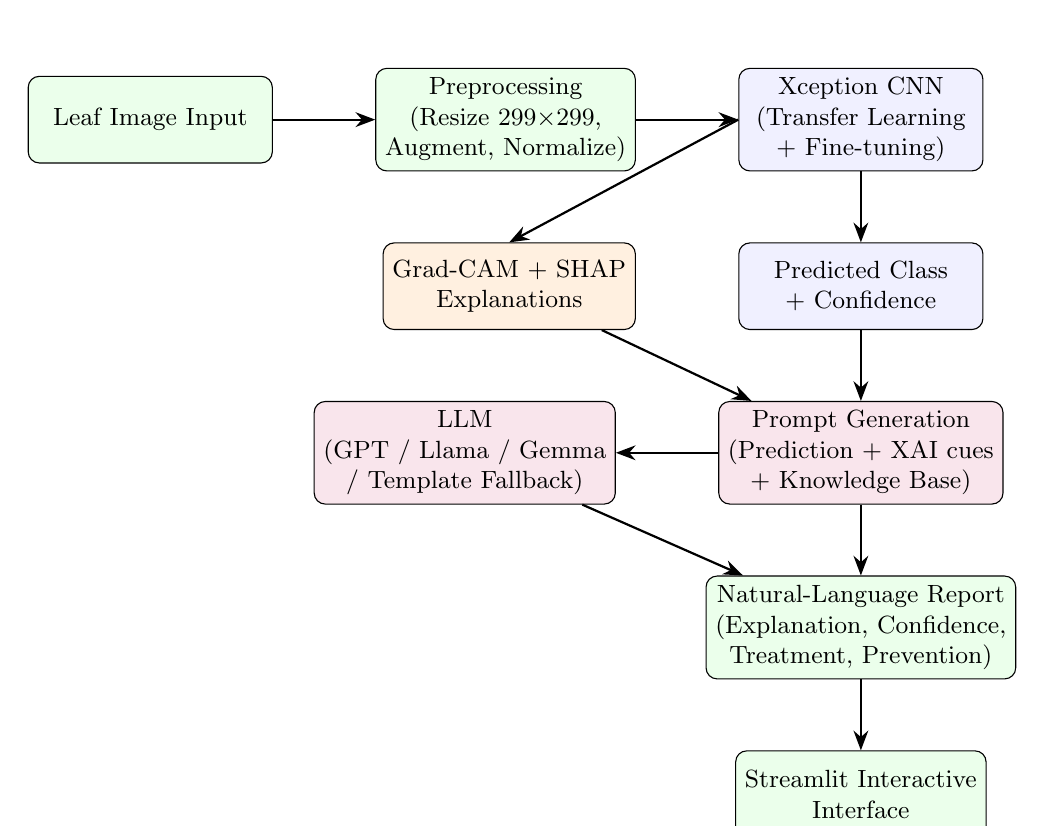
\begin{tikzpicture}[
    node distance=0.9cm and 1.3cm,
    box/.style={draw, rounded corners, minimum width=3.1cm, minimum height=1.1cm, align=center, font=\small, fill=blue!6},
    dbox/.style={draw, rounded corners, minimum width=3.1cm, minimum height=1.1cm, align=center, font=\small, fill=green!8},
    xbox/.style={draw, rounded corners, minimum width=3.1cm, minimum height=1.1cm, align=center, font=\small, fill=orange!12},
    lbox/.style={draw, rounded corners, minimum width=3.1cm, minimum height=1.1cm, align=center, font=\small, fill=purple!10},
    arrow/.style={-{Stealth[length=2.5mm]}, thick}
]
\node[dbox] (input) {Leaf Image Input};
\node[dbox, right=of input] (preprocess) {Preprocessing\\(Resize 299$\times$299,\\Augment, Normalize)};
\node[box, right=of preprocess] (xception) {Xception CNN\\(Transfer Learning\\+ Fine-tuning)};
\node[box, below=of xception] (prediction) {Predicted Class\\+ Confidence};
\node[xbox, left=of prediction] (xai) {Grad-CAM + SHAP\\Explanations};
\node[lbox, below=of prediction] (prompt) {Prompt Generation\\(Prediction + XAI cues\\+ Knowledge Base)};
\node[lbox, left=of prompt] (llm) {LLM\\(GPT / Llama / Gemma\\/ Template Fallback)};
\node[dbox, below=of prompt] (report) {Natural-Language Report\\(Explanation, Confidence,\\Treatment, Prevention)};
\node[dbox, below=of report] (ui) {Streamlit Interactive\\Interface};

\draw[arrow] (input) -- (preprocess);
\draw[arrow] (preprocess) -- (xception);
\draw[arrow] (xception) -- (prediction);
\draw[arrow] (xception.west) -- (xai.north);
\draw[arrow] (prediction) -- (prompt);
\draw[arrow] (xai) -- (prompt);
\draw[arrow] (prompt) -- (llm);
\draw[arrow] (llm) -- (report);
\draw[arrow] (prompt) -- (report);
\draw[arrow] (report) -- (ui);
\end{tikzpicture}
\caption{Overall architecture of the proposed explainable crop disease diagnosis framework.}
\label{fig:architecture}
\end{figure}

\section{Dataset Description}
This research uses the \textbf{New Bangladeshi Crop Disease} dataset, obtained from Kaggle, which contains a
total of \textbf{13,024} leaf images organized into \textbf{14} classes spanning four major crops grown in
Bangladesh: Corn, Potato, Rice, and Wheat. Each class corresponds to either a specific disease or a healthy leaf
of the given crop. Table~\ref{tab:class_distribution} summarizes the number of images available per class.

\begin{table}[H]
\centering
\caption{Class-wise image distribution in the New Bangladeshi Crop Disease dataset.}
\label{tab:class_distribution}
\begin{tabular}{lr}
\toprule
\textbf{Class} & \textbf{Number of Images} \\
\midrule
Corn -- Common Rust & 1{,}192 \\
Corn -- Gray Leaf Spot & 513 \\
Corn -- Healthy & 1{,}162 \\
Corn -- Northern Leaf Blight & 985 \\
Potato -- Early Blight & 1{,}000 \\
Potato -- Healthy & 152 \\
Potato -- Late Blight & 1{,}000 \\
Rice -- Brown Spot & 613 \\
Rice -- Healthy & 1{,}488 \\
Rice -- Leaf Blast & 977 \\
Rice -- Neck Blast & 1{,}000 \\
Wheat -- Brown Rust & 902 \\
Wheat -- Healthy & 1{,}116 \\
Wheat -- Yellow Rust & 924 \\
\midrule
\textbf{Total} & \textbf{13{,}024} \\
\bottomrule
\end{tabular}
\end{table}

As Table~\ref{tab:class_distribution} shows, the dataset exhibits moderate class imbalance -- most notably,
\textit{Potato -- Healthy} contains only 152 images compared with over 1,000 images for several other classes.
This imbalance is addressed during training using class-weighting (Section~\ref{sec:training}). Figure
\ref{fig:class_dist} visualizes this distribution, and Figure~\ref{fig:sample_grid} shows representative sample
images from several classes.

\begin{figure}[H]
\centering

\includegraphics[width=0.95\textwidth]{class_distribution.png}
\caption{Number of images per disease/health class in the dataset.}
\label{fig:class_dist}
\end{figure}

\begin{figure}[H]
\centering

\includegraphics[width=0.85\textwidth]{sample_grid.png}
\caption{Representative sample leaf images from a subset of dataset classes.}
\label{fig:sample_grid}
\end{figure}

\subsection{Train/Validation/Test Split}
The dataset was partitioned using a \textbf{stratified 70/15/15 split}, ensuring that the class proportions in
the original dataset are preserved across the training, validation, and test subsets. This resulted in
\textbf{9,116} training images, \textbf{1,954} validation images, and \textbf{1,954} test images. Stratification
was performed using \texttt{scikit-learn}'s \texttt{train\_test\_split} function with the class label as the
stratification key, applied in two stages (first separating the training set, then splitting the remainder into
validation and test sets). Figure~\ref{fig:split_dist} confirms that class proportions are consistently
maintained across all three subsets.

\begin{figure}[H]
\centering

\includegraphics[width=0.95\textwidth]{split_distribution.png}
\caption{Train / validation / test split per class, confirming stratification.}
\label{fig:split_dist}
\end{figure}

\section{Data Preprocessing}
\subsection{Resizing and Normalization}
All input images were resized to \textbf{299$\times$299} pixels, the native input resolution expected by the
Xception architecture. Pixel intensities were normalized using Xception's associated
\texttt{preprocess\_input} function, which rescales pixel values from the $[0, 255]$ range to $[-1, 1]$, matching
the normalization scheme used when Xception was originally pretrained on ImageNet.

\subsection{Data Augmentation}
To improve generalization and reduce overfitting given the moderate dataset size, on-the-fly data augmentation
was applied to the \textit{training} set only, using Keras's \texttt{ImageDataGenerator}. The augmentation
scheme included:
\begin{itemize}
    \item Random rotation (up to $30^{\circ}$)
    \item Width and height shifts (up to 15\% of image dimensions)
    \item Shear transformation (up to 0.1)
    \item Zoom (up to 20\%)
    \item Brightness adjustment (in the range $[0.8, 1.2]$)
    \item Horizontal flipping
\end{itemize}
No augmentation was applied to the validation or test sets, which were only resized and normalized, ensuring
that reported evaluation metrics reflect performance on realistic, unaltered images. Figure
\ref{fig:augmentation} illustrates the visual effect of the augmentation pipeline on a representative training
image.

\begin{figure}[H]
\centering

\includegraphics[width=0.95\textwidth]{augmentation_examples.png}
\caption{Effect of the data augmentation pipeline on a sample training image.}
\label{fig:augmentation}
\end{figure}

\subsection{Class Imbalance Handling}
Given the class imbalance noted in Table~\ref{tab:class_distribution}, class weights were computed using the
inverse class frequency (via \texttt{scikit-learn}'s \texttt{compute\_class\_weight} with the \texttt{"balanced"}
mode) and supplied to the training loop. This down-weights the contribution of the loss from over-represented
classes (e.g., \textit{Rice -- Healthy}) and up-weights under-represented classes (e.g., \textit{Potato --
Healthy}), encouraging the model to learn discriminative features for minority classes rather than being
dominated by majority-class examples.

\section{Model Architecture}
\label{sec:model_architecture}
The proposed classifier uses \textbf{Xception}~\cite{chollet2017xception}, pretrained on ImageNet, as a
convolutional feature extractor, with a custom classification head appended for the 14-class crop disease
classification task. The full architecture is as follows:
\begin{enumerate}
    \item \textbf{Input layer}: $299 \times 299 \times 3$ RGB image.
    \item \textbf{Xception backbone} (pretrained on ImageNet, top classification layer excluded), producing a
          $10 \times 10 \times 2048$ feature map at its final convolutional layer.
    \item \textbf{Global Average Pooling (GAP)} layer, reducing the feature map to a 2048-dimensional feature
          vector.
    \item \textbf{Batch Normalization} layer.
    \item \textbf{Dense layer} (512 units, ReLU activation).
    \item \textbf{Dropout} layer (rate = 0.4).
    \item \textbf{Dense layer} (256 units, ReLU activation).
    \item \textbf{Dropout} layer (rate = 0.3).
    \item \textbf{Output Dense layer} (14 units, softmax activation), producing class probabilities.
\end{enumerate}

\subsection{Two-Phase Transfer Learning}
Training was conducted in two phases:
\begin{itemize}
    \item \textbf{Phase 1 -- Head-only training}: the entire Xception backbone was frozen, and only the newly
          added classification head was trained, using the Adam optimizer with a learning rate of $1 \times
          10^{-3}$. This phase allows the randomly initialized head to reach a reasonable operating point without
          disturbing the pretrained convolutional filters.
    \item \textbf{Phase 2 -- Fine-tuning}: the top layers of the Xception backbone (from layer index 100 onward)
          were unfrozen, and the entire network was fine-tuned end-to-end using a substantially reduced learning
          rate of $1 \times 10^{-5}$, allowing the model to adapt its higher-level convolutional features to the
          texture, color, and lesion patterns specific to crop disease imagery, while the frozen lower layers
          preserve general-purpose low-level features learned from ImageNet.
\end{itemize}

\subsection{Training Configuration}
\label{sec:training}
The model was trained with the following configuration:
\begin{itemize}
    \item \textbf{Loss function}: categorical cross-entropy.
    \item \textbf{Optimizer}: Adam, with phase-specific learning rates as described above.
    \item \textbf{Batch size}: 32.
    \item \textbf{Class weights}: computed via inverse class frequency, as described in Section 3.4.3 above.
    \item \textbf{EarlyStopping}: monitoring validation loss, with a patience of 6 epochs and restoration of the
          best weights observed during training.
    \item \textbf{ModelCheckpoint}: saving the model with the highest validation accuracy observed during
          training.
    \item \textbf{ReduceLROnPlateau}: reducing the learning rate by a factor of 0.5 when validation loss plateaus
          for 3 consecutive epochs.
\end{itemize}

\section{Evaluation Metrics}
The trained model was evaluated on the held-out test set (1,954 images, never used during training or
validation) using the following standard classification metrics:
\begin{itemize}
    \item \textbf{Accuracy}: the proportion of correctly classified test images.
    \item \textbf{Precision, Recall, and F1-score}: computed per class, and aggregated using both macro-averaging
          (unweighted mean across classes, treating each class equally regardless of support) and
          weighted-averaging (mean weighted by class support, reflecting overall dataset performance).
    \item \textbf{Confusion Matrix}: a $14 \times 14$ matrix showing the distribution of predicted versus true
          class labels, normalized by row (true class) to show per-class recall visually.
    \item \textbf{ROC Curves and AUC}: computed per class using a one-vs-rest strategy, with a macro-averaged AUC
          summarizing overall discriminative performance across all 14 classes.
\end{itemize}

\section{Explainable AI Module}
\label{sec:xai}
To address the opacity of the CNN classifier, two complementary XAI techniques were integrated into the
framework.

\subsection{Grad-CAM}
Grad-CAM~\cite{selvaraju2017gradcam} produces a coarse localization heatmap by computing the gradient of the
predicted class score $y^c$ with respect to the feature maps $A^k$ of the last convolutional layer, and using
global average pooling of these gradients to obtain importance weights $\alpha_k^c$ for each feature map channel
$k$:
\begin{equation}
\alpha_k^c = \frac{1}{Z} \sum_{i}\sum_{j} \frac{\partial y^c}{\partial A^k_{ij}}
\end{equation}
The Grad-CAM heatmap is then obtained as a weighted combination of the forward-pass feature maps, followed by a
ReLU activation to retain only features with a positive influence on the target class:
\begin{equation}
L^c_{\text{Grad-CAM}} = \text{ReLU}\left(\sum_k \alpha_k^c A^k\right)
\end{equation}
The resulting heatmap is resized to the original image dimensions and overlaid on the input leaf image to
visually highlight the regions (e.g., lesions, discoloration) that most influenced the predicted class.

\subsection{SHAP}
SHAP~\cite{lundberg2017shap} attributes to each input feature $i$ a Shapley value $\phi_i$, representing its
average marginal contribution to the model's output across all possible orderings (coalitions) of the input
features:
\begin{equation}
\phi_i = \sum_{S \subseteq F \setminus \{i\}} \frac{|S|!\,(|F|-|S|-1)!}{|F|!} \left[f(S \cup \{i\}) - f(S)\right]
\end{equation}
where $F$ is the full set of input features and $f$ denotes the model's output as a function of a given feature
subset $S$. In this thesis, SHAP's \texttt{GradientExplainer} was used, which approximates Shapley values
efficiently for differentiable models such as CNNs using a small background dataset (50 randomly sampled training
images) to estimate the expected model output baseline.

\subsection{Comparing Grad-CAM and SHAP}
Both explanation methods were computed for the same input image and visualized side by side, alongside a
qualitative \textit{agreement map} obtained by normalizing and multiplying the two attribution maps. Regions
highlighted by both methods provide stronger evidence that the classifier is genuinely attending to disease
symptoms rather than incidental background correlations, serving as a cross-validation step for explanation
reliability.

\section{LLM-Based Natural Language Decision Support}
\label{sec:llm}
The final stage of the pipeline converts the CNN's structured prediction and the XAI-derived visual evidence into
a natural-language diagnostic report, intended to be understandable by a non-technical end user such as a
smallholder farmer.

\subsection{Visual Evidence Summarization}
Grad-CAM and SHAP outputs are first converted into short, human-readable keyword phrases (e.g., \textit{``leaf
lesions, brown color, irregular texture, concentrated lesion region''}) by computing simple image statistics
within the highlighted region: dominant color (via mean RGB values within the mask), boundary irregularity (via
contour perimeter-to-area ratio), and spatial extent (localized versus widespread).

\subsection{Prompt Engineering}
A structured prompt is automatically constructed from: (i) the predicted class and confidence score, (ii) the
visual evidence keywords derived above, and (iii) a short reference entry from a compact agronomic knowledge
base containing typical symptoms, treatment, and prevention guidance for the predicted disease class. The
knowledge base grounds the LLM's response, reducing the risk of hallucinated or agronomically incorrect
recommendations. The prompt instructs the LLM to produce exactly four sections: \textit{Disease Explanation},
\textit{Confidence Interpretation}, \textit{Recommended Treatment}, and \textit{Preventive Measures}, using
simple, non-technical language suitable for a farmer audience.

\subsection{LLM Backend}
The framework supports three interchangeable backends for natural language generation:
\begin{enumerate}
    \item \textbf{OpenAI GPT} (via the OpenAI API), used when an API key is available.
    \item \textbf{Local Llama-3 / Gemma} models (via the Hugging Face \texttt{transformers} library, or an
          \texttt{ollama} server), enabling fully offline operation suitable for low-connectivity rural
          deployment.
    \item \textbf{Rule-based template fallback}, which populates the same four-section report structure directly
          from the knowledge base and a confidence-interpretation heuristic, guaranteeing that the system remains
          fully functional even without any external LLM access.
\end{enumerate}
This tiered design ensures the framework degrades gracefully: if no LLM backend is available (e.g., in a
disconnected field environment), the template fallback still produces a complete, structured diagnostic report.

\section{System Implementation}
The complete pipeline -- classification, Grad-CAM, SHAP, and LLM-based report generation -- was wrapped into a
single function and exposed through an interactive \textbf{Streamlit} web application. The application allows a
user to upload a leaf photograph and receive, in a single view: the predicted disease class and confidence score,
the Grad-CAM heatmap overlay, the SHAP attribution map, and the full natural-language diagnostic report, which can
be downloaded as a text file. The backend was implemented in Python using TensorFlow/Keras for model training and
inference, OpenCV and Matplotlib for image processing and visualization, and the SHAP library for Shapley-value
computation.

% ============================================================
% CHAPTER 4: RESULTS AND DISCUSSION
% ============================================================
\chapter{Results and Discussion}
\label{ch:results}

\section{Training Performance}
Figure~\ref{fig:training_curves} shows the training and validation accuracy and loss curves across both training
phases. The vertical dashed line marks the transition from Phase 1 (head-only training) to Phase 2 (fine-tuning).
Validation accuracy improved substantially once fine-tuning began, and both EarlyStopping and
ModelCheckpoint ensured that the final evaluated model corresponds to the epoch with the best validation
performance, mitigating overfitting.

\begin{figure}[H]
\centering

\includegraphics[width=0.98\textwidth]{training_curves.png}
\caption{Training and validation accuracy and loss curves across both training phases.}
\label{fig:training_curves}
\end{figure}

\section{Classification Performance}
The fine-tuned model was evaluated on the held-out test set of 1,954 images. Table~\ref{tab:overall_metrics}
summarizes the overall test-set performance.

\begin{table}[H]
\centering
\caption{Overall test-set classification performance.}
\label{tab:overall_metrics}
\begin{tabular}{lr}
\toprule
\textbf{Metric} & \textbf{Value} \\
\midrule
Test Accuracy & 92.27\% \\
Macro-averaged Precision & 0.9101 \\
Macro-averaged Recall & 0.9140 \\
Macro-averaged F1-score & 0.9108 \\
Weighted-averaged Precision & 0.9251 \\
Weighted-averaged Recall & 0.9227 \\
Weighted-averaged F1-score & 0.9229 \\
Macro-averaged ROC-AUC (14 classes) & 0.9969 \\
\bottomrule
\end{tabular}
\end{table}

The model achieves a strong overall test accuracy of 92.27\%, with a macro-averaged ROC-AUC of 0.997 indicating
excellent overall discriminative capability across all 14 classes, even those with fewer training examples.
Table~\ref{tab:per_class_metrics} presents the full per-class precision, recall, and F1-score, computed on the
test set.

\begin{table}[H]
\centering
\caption{Per-class precision, recall, and F1-score on the test set.}
\label{tab:per_class_metrics}
\begin{tabular}{lrrrr}
\toprule
\textbf{Class} & \textbf{Precision} & \textbf{Recall} & \textbf{F1-score} & \textbf{Support} \\
\midrule
Corn -- Common Rust          & 0.994 & 1.000 & 0.997 & 179 \\
Corn -- Gray Leaf Spot        & 0.745 & 0.909 & 0.819 & 77 \\
Corn -- Healthy               & 0.977 & 0.994 & 0.986 & 174 \\
Corn -- Northern Leaf Blight  & 0.946 & 0.830 & 0.884 & 147 \\
Potato -- Early Blight        & 1.000 & 0.987 & 0.993 & 150 \\
Potato -- Healthy             & 0.870 & 0.870 & 0.870 & 23 \\
Potato -- Late Blight         & 0.967 & 0.980 & 0.974 & 150 \\
Rice -- Brown Spot            & 0.686 & 0.761 & 0.722 & 92 \\
Rice -- Healthy               & 0.853 & 0.861 & 0.857 & 223 \\
Rice -- Leaf Blast            & 0.785 & 0.721 & 0.752 & 147 \\
Rice -- Neck Blast            & 1.000 & 1.000 & 1.000 & 150 \\
Wheat -- Brown Rust           & 0.992 & 0.919 & 0.954 & 136 \\
Wheat -- Healthy              & 0.955 & 1.000 & 0.977 & 168 \\
Wheat -- Yellow Rust          & 0.971 & 0.964 & 0.967 & 138 \\
\midrule
\textbf{Macro average}   & \textbf{0.910} & \textbf{0.914} & \textbf{0.911} & 1{,}954 \\
\textbf{Weighted average} & \textbf{0.925} & \textbf{0.923} & \textbf{0.923} & 1{,}954 \\
\bottomrule
\end{tabular}
\end{table}

Several classes -- notably \textit{Rice -- Neck Blast} (F1 = 1.000), \textit{Corn -- Common Rust} (F1 = 0.997),
and \textit{Potato -- Early Blight} (F1 = 0.993) -- are classified almost perfectly. In contrast, \textit{Rice --
Brown Spot} (F1 = 0.722) and \textit{Rice -- Leaf Blast} (F1 = 0.752) show comparatively lower performance,
suggesting visual similarity between these two rice diseases that the model occasionally confuses (further
examined via the confusion matrix in Section~\ref{sec:confmatrix}). \textit{Potato -- Healthy} also shows
comparatively lower performance (F1 = 0.870), likely attributable to its small support in the test set (only 23
images), corresponding to the class imbalance noted in Table~\ref{tab:class_distribution}.

\section{Confusion Matrix Analysis}
\label{sec:confmatrix}
Figure~\ref{fig:confusion_matrix} presents the row-normalized confusion matrix on the test set, where each cell
represents the proportion of a given true class predicted as each possible class.

\begin{figure}[H]
\centering

\includegraphics[width=0.85\textwidth]{confusion_matrix.png}
\caption{Row-normalized confusion matrix on the test set.}
\label{fig:confusion_matrix}
\end{figure}

Consistent with the per-class metrics in Table~\ref{tab:per_class_metrics}, the confusion matrix reveals that the
majority of the model's residual errors occur between \textit{Rice -- Brown Spot} and \textit{Rice -- Leaf
Blast}, both of which present as brownish, roughly circular-to-elongated lesions on rice leaves and can be
visually similar, particularly under variable lighting or at an early disease stage. This finding suggests that
future work could benefit from additional training images specifically capturing the visually distinguishing
features between these two diseases (e.g., the more elongated, gray-centered lesions characteristic of leaf
blast versus the smaller, more circular lesions of brown spot).

\section{ROC Curve and AUC Analysis}
Figure~\ref{fig:roc_curves} shows the one-vs-rest ROC curves for a representative subset of classes, together
with the macro-averaged ROC curve across all 14 classes.

\begin{figure}[H]
\centering

\includegraphics[width=0.85\textwidth]{roc_curves.png}
\caption{One-vs-rest ROC curves for a representative subset of classes, with macro-average.}
\label{fig:roc_curves}
\end{figure}

The macro-averaged AUC of 0.997 indicates that, even for classes with relatively lower F1-scores (such as
\textit{Rice -- Brown Spot} and \textit{Rice -- Leaf Blast}), the model's predicted class probabilities remain
highly discriminative in a ranking sense; the comparatively lower F1-scores for these classes are therefore
better attributed to confusion between two specific, visually similar classes at the operating threshold, rather
than a general failure to learn discriminative features for those classes.

\section{Explainability Results}
\subsection{Grad-CAM Visualization}
Figure~\ref{fig:gradcam_demo} shows a representative Grad-CAM visualization for a test image, comprising the
original image, the raw heatmap, and the heatmap overlaid on the original leaf image.

\begin{figure}[H]
\centering

\includegraphics[width=0.98\textwidth]{gradcam_demo.png}
\caption{Grad-CAM visualization for a representative test image: original image, heatmap, and overlay.}
\label{fig:gradcam_demo}
\end{figure}

The Grad-CAM overlay consistently localizes attention to visually diseased or discolored regions of the leaf
surface, rather than to background elements, supporting the conclusion that the classifier is basing its
predictions on genuine disease-relevant visual features.

\subsection{SHAP Explanation}
Figure~\ref{fig:shap_demo} shows the corresponding SHAP attribution map for the same test image, computed using
\texttt{GradientExplainer} with a 50-image background sample.

\begin{figure}[H]
\centering

\includegraphics[width=0.75\textwidth]{shap_demo.png}
\caption{SHAP attribution map for a representative test image.}
\label{fig:shap_demo}
\end{figure}

\subsection{Comparing Grad-CAM and SHAP}
Figure~\ref{fig:explanation_comparison} places the original image, Grad-CAM overlay, SHAP attribution map, and a
qualitative agreement map side by side for direct comparison.

\begin{figure}[H]
\centering

\includegraphics[width=0.98\textwidth]{explanation_comparison.png}
\caption{Side-by-side comparison of Grad-CAM and SHAP explanations, with a qualitative agreement map.}
\label{fig:explanation_comparison}
\end{figure}

The two explanation methods broadly agree on the diseased leaf regions driving the model's prediction, despite
being derived from fundamentally different mathematical principles (gradient-based localization versus
Shapley-value attribution). This cross-method agreement increases confidence that the classifier's decisions are
grounded in genuine disease symptomatology rather than spurious correlations with background or imaging
artifacts, directly supporting Objective 3 and Objective 6 of this research.

\section{LLM-Based Decision Support Output}
Table~\ref{tab:llm_sample} presents two representative, end-to-end examples generated by the framework's
interactive prediction pipeline (Section~\ref{sec:llm}), each combining the CNN's prediction, the summarized
visual evidence, and the resulting natural-language report (generated here via the rule-based template backend).

\begin{table}[H]
\centering
\caption{Representative end-to-end diagnostic outputs generated by the framework.}
\label{tab:llm_sample}
\small
\begin{tabular}{p{2.6cm}p{2.0cm}p{8.5cm}}
\toprule
\textbf{Prediction} & \textbf{Confidence} & \textbf{Generated Report (abridged)} \\
\midrule
Rice -- Healthy & 98.4\% &
\textit{Disease Explanation}: leaf shows characteristics consistent with a healthy leaf surface.
\textit{Confidence Interpretation}: very high confidence -- visual evidence strongly supports this diagnosis.
\textit{Recommended Treatment}: no treatment required; continue routine monitoring.
\textit{Preventive Measures}: maintain balanced fertilization and proper field drainage; monitor regularly for
early symptoms. \\
\addlinespace
Corn -- Common Rust & 100.0\% &
\textit{Disease Explanation}: leaf shows lesions and discoloration consistent with Common Rust.
\textit{Confidence Interpretation}: very high confidence -- visual evidence strongly and unambiguously supports
this diagnosis.
\textit{Recommended Treatment}: consult local agricultural extension services for a disease-specific
fungicide/pesticide recommendation; remove and destroy infected plant material to reduce spread.
\textit{Preventive Measures}: use disease-resistant varieties where available; practice crop rotation; maintain
balanced fertilization and field drainage. \\
\bottomrule
\end{tabular}
\end{table}

These examples demonstrate that the framework successfully converts a raw softmax prediction and confidence score
into an actionable, structured, natural-language report -- directly fulfilling Objective 4 and Objective 5 of
this research. Figure~\ref{fig:interactive_demo} shows a complete example from the interactive prediction
pipeline, combining the original leaf image, its Grad-CAM heatmap, and its SHAP explanation in a single view.

\begin{figure}[H]
\centering

\includegraphics[width=0.98\textwidth]{interactive_demo_result.png}
\caption{Complete end-to-end interactive prediction output: input image, Grad-CAM heatmap, and SHAP explanation.}
\label{fig:interactive_demo}
\end{figure}

\section{Discussion}
The experimental results address each of the six specific objectives outlined in Chapter~1. The fine-tuned
Xception classifier (Objective 1) achieves a strong overall test accuracy of 92.27\%, evaluated comprehensively
using accuracy, per-class and aggregate precision/recall/F1-score, a confusion matrix, and ROC-AUC analysis
(Objective 2). The integration of Grad-CAM and SHAP (Objective 3) provides complementary, largely consistent
visual explanations that increase confidence in the model's decision-making process. The LLM-based natural
language module (Objective 4) successfully translates the model's technical output into structured,
farmer-friendly reports, and the accompanying agronomic knowledge base grounds the generated treatment and
prevention recommendations (Objective 5). Taken together, these components form a framework that is substantially
more transparent and usable than a standalone classifier (Objective 6), though a formal user study with farmers
and agricultural extension officers -- outside the scope of this thesis -- would be needed to rigorously quantify
improvements in trust and usability.

The main performance limitation observed is confusion between \textit{Rice -- Brown Spot} and \textit{Rice --
Leaf Blast}, two visually similar diseases. Given that the macro-averaged AUC remains very high (0.997), this
appears to be a threshold/ranking issue for a specific pair of classes rather than a fundamental failure of
feature learning, and could likely be mitigated through additional training data, targeted data augmentation, or
a hierarchical classification scheme that first identifies the crop and then the specific disease. The current
LLM-based decision-support module also relies on an illustrative agronomic knowledge base covering a subset of
classes; a production deployment would require this knowledge base to be extended and validated against
authoritative sources (e.g., the Bangladesh Department of Agricultural Extension) for every disease class in the
dataset.

% ============================================================
% CHAPTER 5: CONCLUSION AND FUTURE WORK
% ============================================================
\chapter{Conclusion and Future Work}
\label{ch:conclusion}

\section{Conclusion}
This thesis presented an explainable, LLM-supported crop disease diagnosis framework for Bangladeshi agriculture,
combining a fine-tuned Xception CNN classifier, dual explainability via Grad-CAM and SHAP, and an LLM-based
natural language decision-support module. Evaluated on the New Bangladeshi Crop Disease dataset (13,024 images
across 14 classes spanning Corn, Potato, Rice, and Wheat), the proposed classifier achieved a test accuracy of
92.27\%, a macro-averaged F1-score of 0.911, and a macro-averaged ROC-AUC of 0.997. Grad-CAM and SHAP explanations
were found to largely agree on the diseased leaf regions driving each prediction, supporting the reliability of
the underlying classification decisions. A prompt-engineering pipeline, grounded in a compact agronomic knowledge
base, successfully converted the model's structured predictions into natural-language diagnostic reports covering
disease explanation, confidence interpretation, treatment, and prevention, with the flexibility to use OpenAI
GPT, local Llama-3/Gemma models, or a fully offline rule-based template fallback. The complete framework was
deployed as an interactive Streamlit web application, demonstrating an end-to-end, farmer-facing decision-support
tool. Collectively, these results demonstrate that combining an accurate CNN classifier with XAI and LLM-based
natural language generation can meaningfully improve the transparency, interpretability, and practical usability
of AI-assisted crop disease diagnosis.

\section{Limitations}
This research has several limitations that should be considered when interpreting its results. First, the
dataset, while reasonably large (13,024 images), is limited to 14 classes across four crops; many other crops and
diseases economically important in Bangladesh are not represented. Second, the dataset images may not fully
capture the diversity of lighting, background, and image-capture conditions encountered in real farm-field
deployment, raising the possibility of domain shift when the model is applied to genuinely new field photographs.
Third, the illustrative agronomic knowledge base used to ground the LLM's recommendations covers only a subset of
disease classes in detail; a production system would require comprehensive, expert-validated coverage of every
class. Fourth, while Grad-CAM and SHAP were shown to agree qualitatively on diseased regions, this agreement does
not constitute formal proof of the specific biological mechanism underlying a diagnosis, and both techniques
should be understood as supporting evidence rather than definitive causal explanations. Finally, no formal user
study with farmers or agricultural extension officers was conducted to quantitatively assess improvements in
trust and usability resulting from the added explainability and natural-language reporting.

\section{Future Work}
Building on the findings and limitations of this thesis, several directions for future work are identified:
\begin{itemize}
    \item \textbf{Dataset expansion}: collecting field-captured images directly from Bangladeshi farms, under
          varied lighting and background conditions, to reduce domain shift and extend disease/crop coverage
          beyond the current 14 classes.
    \item \textbf{Knowledge base validation}: expanding and validating the agronomic knowledge base against
          authoritative sources such as the Bangladesh Department of Agricultural Extension (DAE), the
          Bangladesh Rice Research Institute (BRRI), and the Bangladesh Agricultural Research Institute (BARI).
    \item \textbf{Human evaluation study}: conducting a formal study with farmers and agricultural extension
          officers to assess the framework's practical impact on trust, comprehension, and decision quality,
          compared with a non-explainable baseline.
    \item \textbf{On-device deployment}: converting the trained model to a lightweight, quantized format (e.g.,
          TensorFlow Lite) for offline, on-device inference on low-cost smartphones in areas with limited
          internet connectivity.
    \item \textbf{Confusable-class refinement}: targeted data collection and, potentially, a hierarchical
          classification scheme to specifically address the observed confusion between \textit{Rice -- Brown
          Spot} and \textit{Rice -- Leaf Blast}.
    \item \textbf{Multimodal LLM integration}: exploring vision-language models capable of reasoning directly
          over leaf images, rather than relying solely on keyword summaries of Grad-CAM/SHAP outputs, potentially
          enabling richer, more precisely grounded natural-language explanations.
\end{itemize}

% ============================================================
% REFERENCES
% ============================================================
\begin{thebibliography}{99}

\bibitem{mohanty2016}
Mohanty, S. P., Hughes, D. P., \& Salath\'{e}, M. (2016). Using deep learning for image-based plant disease
detection. \textit{Frontiers in Plant Science}, 7, 1419.

\bibitem{ferentinos2018}
Ferentinos, K. P. (2018). Deep learning models for plant disease detection and diagnosis. \textit{Computers and
Electronics in Agriculture}, 145, 311--318.

\bibitem{deng2009imagenet}
Deng, J., Dong, W., Socher, R., Li, L.-J., Li, K., \& Fei-Fei, L. (2009). ImageNet: A large-scale hierarchical
image database. In \textit{Proceedings of the IEEE Conference on Computer Vision and Pattern Recognition (CVPR)},
248--255.

\bibitem{simonyan2014vgg}
Simonyan, K., \& Zisserman, A. (2014). Very deep convolutional networks for large-scale image recognition.
\textit{arXiv preprint arXiv:1409.1556}.

\bibitem{he2016resnet}
He, K., Zhang, X., Ren, S., \& Sun, J. (2016). Deep residual learning for image recognition. In
\textit{Proceedings of the IEEE Conference on Computer Vision and Pattern Recognition (CVPR)}, 770--778.

\bibitem{chollet2017xception}
Chollet, F. (2017). Xception: Deep learning with depthwise separable convolutions. In \textit{Proceedings of the
IEEE Conference on Computer Vision and Pattern Recognition (CVPR)}, 1251--1258.

\bibitem{selvaraju2017gradcam}
Selvaraju, R. R., Cogswell, M., Das, A., Vedantam, R., Parikh, D., \& Batra, D. (2017). Grad-CAM: Visual
explanations from deep networks via gradient-based localization. In \textit{Proceedings of the IEEE International
Conference on Computer Vision (ICCV)}, 618--626.

\bibitem{lundberg2017shap}
Lundberg, S. M., \& Lee, S.-I. (2017). A unified approach to interpreting model predictions. In \textit{Advances
in Neural Information Processing Systems (NeurIPS)}, 30.

\bibitem{ribeiro2016lime}
Ribeiro, M. T., Singh, S., \& Guestrin, C. (2016). ``Why should I trust you?'': Explaining the predictions of any
classifier. In \textit{Proceedings of the 22nd ACM SIGKDD International Conference on Knowledge Discovery and
Data Mining}, 1135--1144.

\bibitem{vaswani2017attention}
Vaswani, A., Shazeer, N., Parmar, N., Uszkoreit, J., Jones, L., Gomez, A. N., Kaiser, {\L}., \& Polosukhin, I.
(2017). Attention is all you need. In \textit{Advances in Neural Information Processing Systems (NeurIPS)}, 30.

\bibitem{brown2020gpt3}
Brown, T., Mann, B., Ryder, N., Subbiah, M., Kaplan, J. D., Dhariwal, P., et al. (2020). Language models are
few-shot learners. In \textit{Advances in Neural Information Processing Systems (NeurIPS)}, 33, 1877--1901.

\bibitem{touvron2023llama}
Touvron, H., Lavril, T., Izacard, G., Martinet, X., Lachaux, M.-A., Lacroix, T., et al. (2023). LLaMA: Open and
efficient foundation language models. \textit{arXiv preprint arXiv:2302.13971}.

\end{thebibliography}
\addcontentsline{toc}{chapter}{References}

% ============================================================
% APPENDIX
% ============================================================
\appendix
\chapter{Selected Source Code Listings}
\label{ap:code}

This appendix presents selected, representative code listings from the implementation. The complete
implementation, including the full data pipeline, training loop, evaluation code, XAI modules, and the LLM-based
decision-support module, is available in the accompanying Jupyter notebook and Streamlit application.

\section{Xception Model Construction and Two-Phase Transfer Learning}
\begin{lstlisting}[caption={Model construction with configurable backbone freezing for two-phase transfer learning.}]
def build_model(num_classes, img_size, fine_tune_at=None):
    base_model = Xception(
        weights="imagenet",
        include_top=False,
        input_shape=(*img_size, 3),
    )

    if fine_tune_at is None:
        base_model.trainable = False        # Phase 1: fully frozen
    else:
        base_model.trainable = True
        for layer in base_model.layers[:fine_tune_at]:
            layer.trainable = False         # Phase 2: unfreeze top blocks only

    inputs = keras.Input(shape=(*img_size, 3))
    x = base_model(inputs, training=False if fine_tune_at is None else None)
    x = layers.GlobalAveragePooling2D(name="gap")(x)
    x = layers.BatchNormalization()(x)
    x = layers.Dense(512, activation="relu")(x)
    x = layers.Dropout(0.4)(x)
    x = layers.Dense(256, activation="relu")(x)
    x = layers.Dropout(0.3)(x)
    outputs = layers.Dense(num_classes, activation="softmax", name="predictions")(x)

    model = keras.Model(inputs, outputs, name="Xception_BD_CropDisease")
    return model, base_model
\end{lstlisting}

\section{Grad-CAM Heatmap Generation}
\begin{lstlisting}[caption={Grad-CAM heatmap computation using a gradient tape over the last convolutional layer.}]
def make_gradcam_heatmap(img_array, model, last_conv_layer_name, pred_index=None):
    backbone = model.get_layer("xception")
    conv_layer = backbone.get_layer(last_conv_layer_name)
    conv_and_backbone_output_model = keras.models.Model(
        backbone.input, [conv_layer.output, backbone.output]
    )

    head_layers, seen_backbone = [], False
    for layer in model.layers:
        if layer.name == "xception":
            seen_backbone = True
            continue
        if seen_backbone:
            head_layers.append(layer)

    with tf.GradientTape() as tape:
        conv_outputs, backbone_features = conv_and_backbone_output_model(
            img_array, training=False
        )
        tape.watch(conv_outputs)
        x = backbone_features
        for layer in head_layers:
            x = layer(x, training=False)
        predictions = x
        if pred_index is None:
            pred_index = tf.argmax(predictions[0])
        class_channel = predictions[:, pred_index]

    grads = tape.gradient(class_channel, conv_outputs)
    pooled_grads = tf.reduce_mean(grads, axis=(0, 1, 2))
    conv_outputs = conv_outputs[0]
    heatmap = conv_outputs @ pooled_grads[..., tf.newaxis]
    heatmap = tf.squeeze(heatmap)
    heatmap = tf.maximum(heatmap, 0) / (tf.math.reduce_max(heatmap) + 1e-8)
    return heatmap.numpy(), int(pred_index), predictions.numpy()[0]
\end{lstlisting}

\section{LLM Prompt Construction}
\begin{lstlisting}[caption={Automatic prompt construction from model prediction, confidence, and XAI-derived visual evidence.}]
def build_llm_prompt(predicted_class, confidence_pct, crop_name,
                      shap_keywords, gradcam_note):
    kb = get_kb_entry(predicted_class)
    confidence_note = interpret_confidence(confidence_pct)

    prompt = f"""You are an agricultural plant-pathology assistant helping a
Bangladeshi farmer understand an AI-based crop disease diagnosis. Respond in
clear, simple, non-technical language.

STRUCTURED MODEL OUTPUT:
- Crop: {crop_name}
- Predicted disease class: {predicted_class.replace('_', ' ')}
- Model confidence: {confidence_pct:.1f}%
- Grad-CAM visual evidence: {gradcam_note}
- SHAP key visual cues: {shap_keywords}

REFERENCE AGRONOMIC KNOWLEDGE (for grounding only):
- Typical symptoms: {kb['symptoms']}
- General treatment guidance: {kb['treatment']}
- General prevention guidance: {kb['prevention']}

Produce a report with exactly these four sections:
1. Disease Explanation
2. Confidence Interpretation
3. Recommended Treatment
4. Preventive Measures
"""
    return prompt
\end{lstlisting}

\end{document}
